This chapter distinguishes a small candidate-pair smoke fixture from a final evaluation of
answer reuse. The figures and tables below are generated from repository scripts and recorded
CSV files. They do not establish a production error rate, a formal risk guarantee, or an
original algorithmic result. The default gateway mode is exact matching; semantic matching
is an opt-in experimental mode.

\section{Functional Checks}
The default local pytest summary is generated from pytest's JUnit XML. Skipped integration
tests need a disposable Redis Stack; the repository's CI exercises that path separately.
These counts are functional-check evidence, not a statistical quality result.

% Generated by scripts/export_report_tables.py; edit the source CSV, not this file.
\begin{table}[H]
\centering
\footnotesize
\caption{Default local pytest run; skipped integration tests require a disposable Redis Stack.}
\label{tab:checks}
\begin{tabular}{|r|r|r|r|}
\hline
Passed & Skipped & Failures & Errors \\ \hline
83 & 4 & 0 & 0 \\ \hline
\end{tabular}
\end{table}


\section{Candidate-Pair Smoke Fixture}
The input to this experiment is a stored query and an incoming query, labelled by whether
they were intended to be paraphrases. It does not include the actual cached answer or a
human judgement that the answer remains usable. The experiment calls the same
\texttt{CachePolicy.decide} function used by the gateway, but passes zero neighbourhood
density and always supplies the designated stored query as the candidate. It therefore
tests a decision rule in isolation, not candidate retrieval or a changing cache.

Positive recall divides accepted positive pairs by all positive pairs. Negative acceptance
divides accepted negative pairs by all negative pairs. Precision divides accepted positive
pairs by all accepted pairs and is undefined when there are no accepts. Neither positive
recall nor negative acceptance is an end-to-end workload cache-hit or monetary-savings rate.

% Generated by scripts/export_report_tables.py; edit the source CSV, not this file.
\begin{table}[H]
\centering
\footnotesize
\caption{Candidate-pair smoke fixture. Positive recall and negative acceptance use different denominators; this is not workload hit rate or monetary savings.}
\label{tab:ablation}
\begin{tabular}{|l|c|c|c|c|}
\hline
System & Positive recall & Negative acceptance & Precision & Accepted \\ \hline
Baseline (static T=0.72) & 40.0\% & 46.7\% & 46.2\% & 13 \\ \hline
+ Adaptive T & 33.3\% & 33.3\% & 50.0\% & 10 \\ \hline
+ Verifier (Tier-1) & 0.0\% & 0.0\% & N/A & 0 \\ \hline
VeriGate (Tier-1) & 0.0\% & 0.0\% & N/A & 0 \\ \hline
\end{tabular}
\end{table}


The current fixture is deliberately small and was used during development. Thresholds and
heuristic weights were not selected on a separate validation split. The displayed differences
are descriptive results on this fixture; they cannot establish generalisation or a fair
comparison with published systems.

\begin{figure}[H]
\centering
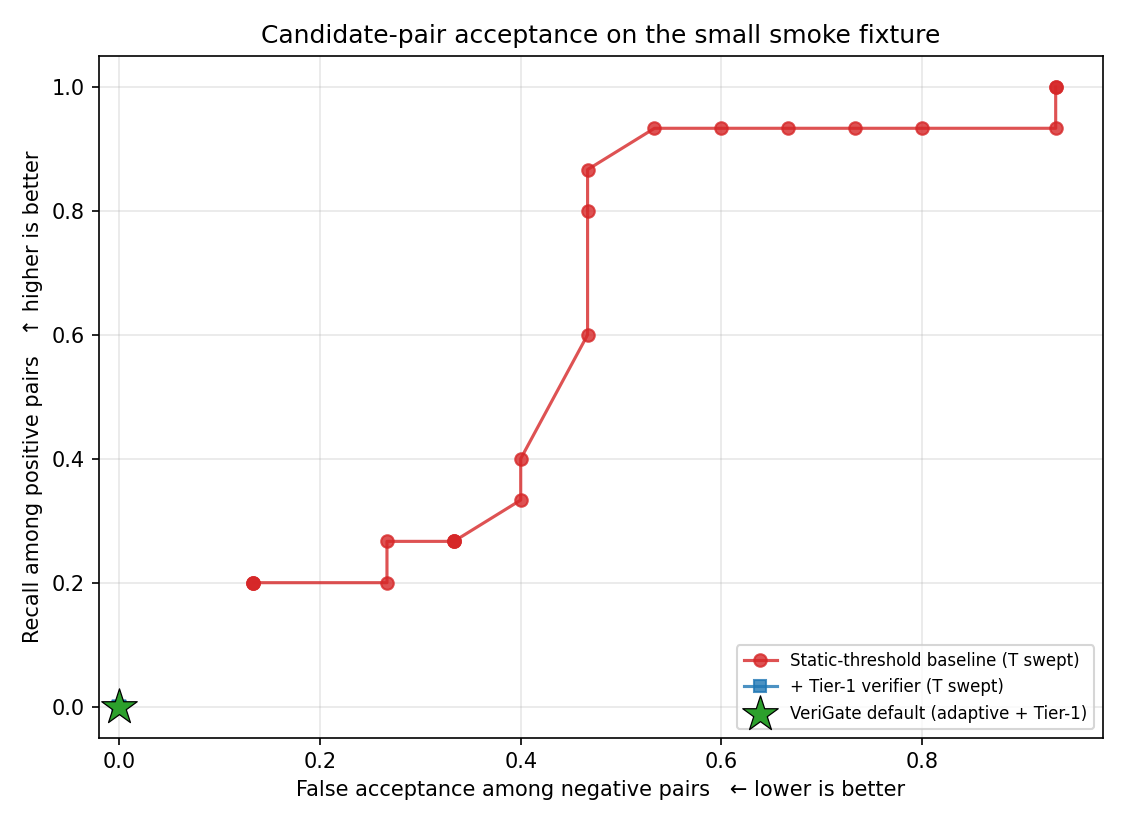
\includegraphics[width=0.82\textwidth,keepaspectratio]{tradeoff.png}
\caption{Threshold sweep on the candidate-pair smoke fixture. Axes are negative-pair
acceptance and positive-pair recall, not real workload risk and savings.}
\end{figure}

\section{Public Query-Pair Proxy Experiments}
Separate scripts load QQP, PAWS, and STS-B query or sentence pairs and keep repeated
normalized queries in the same train, validation, calibration, or test group. Five fixed
seeds evaluate learned accept scorers and transfer. The model was trained on QQP, so PAWS
is a distribution-shift challenge. The table gives the mean per-seed coverage and false
\emph{pair} acceptance among served pairs; it does not say whether a specific cached
answer would have satisfied a request. The strong deterioration on PAWS is a negative
result, not evidence that learned semantic reuse is ready to deploy.

% Generated by scripts/export_report_tables.py; edit the source CSV, not this file.
\begin{table}[H]
\centering
\footnotesize
\caption{Five-seed query-pair proxy transfer; false acceptance is among accepted pairs, not answers.}
\label{tab:learned-proxy}
\begin{tabular}{|l|l|r|r|}
\hline
Test source & Model & Coverage & False pair acceptance \\ \hline
paws & gradient\_boosting & 64.7\% & 52.6\% \\ \hline
paws & logistic\_all & 91.2\% & 55.5\% \\ \hline
qqp & gradient\_boosting & 36.4\% & 29.8\% \\ \hline
qqp & logistic\_all & 36.9\% & 26.6\% \\ \hline
\end{tabular}
\end{table}


A chronological replay fills tenant-partitioned caches under TTL and LRU constraints.
It exercises real neighbourhood density. The source dataset only labels the designated
pair; when retrieval crosses pairs, the outcome is marked unknown rather than correct.
The replay counts below therefore cannot be converted into a true workload answer-error
rate or a monetary saving claim.

% Generated by scripts/export_report_tables.py; edit the source CSV, not this file.
\begin{table}[H]
\centering
\footnotesize
\caption{Chronological QQP pair-proxy replay; unknown cross-pair outcomes are not counted as correct.}
\label{tab:stream-proxy}
\begin{tabular}{|r|l|r|r|r|}
\hline
Capacity & Policy & Known accepts & Known false & Unknown accepts \\ \hline
10 & exact & 706 & 0 & 0 \\ \hline
10 & static\_0.72 & 722 & 88 & 2 \\ \hline
10 & adaptive\_tier1 & 717 & 87 & 0 \\ \hline
100 & exact & 925 & 0 & 0 \\ \hline
100 & static\_0.72 & 980 & 145 & 1 \\ \hline
100 & adaptive\_tier1 & 954 & 99 & 0 \\ \hline
\end{tabular}
\end{table}


An exact binomial upper bound with a finite threshold grid was exercised on synthetic IID
data. The table records how often a nonempty threshold was selected and whether its
known synthetic true risk exceeded the target. Reject-all runs have zero coverage and no
defined conditional risk. Public QQP-to-PAWS pair-proxy calibration selected reject-all
at the tested targets, so it gives no evidence of a useful answer-level guarantee.

% Generated by scripts/export_report_tables.py; edit the source CSV, not this file.
\begin{table}[H]
\centering
\footnotesize
\caption{Synthetic IID bound exercise; reject-all runs have no defined conditional risk.}
\label{tab:risk-synthetic}
\begin{tabular}{|r|r|r|r|}
\hline
Target & Runs & Nonempty selections & True-risk violations \\ \hline
0.5\% & 50 & 0 & 0 \\ \hline
1.0\% & 50 & 0 & 0 \\ \hline
2.0\% & 50 & 35 & 0 \\ \hline
5.0\% & 50 & 50 & 0 \\ \hline
\end{tabular}
\end{table}


\section{Stage and Backend Timings}
The following archived timing CSV files were produced by the repository's latency and
backend scripts. They are stage measurements on a particular machine, not an end-to-end
service-level objective. The backend experiment did not measure the crossover size or
retrieval recall; no scaling claim follows from it.

% Generated by scripts/export_report_tables.py; edit the source CSV, not this file.
\begin{table}[H]
\centering
\footnotesize
\caption{Recorded stage timings in milliseconds; these are not end-to-end provider latency.}
\label{tab:latency}
\begin{tabular}{|l|r|r|r|}
\hline
Stage & p50 & p95 & p99 \\ \hline
embed & 46.51 & 136.69 & 348.71 \\ \hline
knn\_n10 & 0.05 & 0.06 & 1.12 \\ \hline
knn\_n100 & 0.05 & 0.06 & 0.13 \\ \hline
knn\_n500 & 0.08 & 0.14 & 0.19 \\ \hline
knn\_n1000 & 0.12 & 0.22 & 0.33 \\ \hline
knn\_n2000 & 0.34 & 0.71 & 0.90 \\ \hline
tier1\_verify & 0.03 & 0.04 & 0.07 \\ \hline
tier2\_nli & 364.99 & 882.55 & 1761.56 \\ \hline
hit\_tier1\_n1000 & 29.96 & 47.59 & 61.88 \\ \hline
\end{tabular}
\end{table}

% Generated by scripts/export_report_tables.py; edit the source CSV, not this file.
\begin{table}[H]
\centering
\footnotesize
\caption{Recorded lookup p50 latency in milliseconds; the crossover size was not measured.}
\label{tab:backend}
\begin{tabular}{|r|r|r|}
\hline
Entries & In-process & RediSearch \\ \hline
1000 & 0.03 & 3.82 \\ \hline
5000 & 0.20 & 4.16 \\ \hline
10000 & 0.22 & 5.58 \\ \hline
\end{tabular}
\end{table}


\section{Illustrative Cascade Experiment}
The cascade experiment uses a hand-labelled easy/hard query list and an assumed relative
price for weak and strong providers. Its quality metric is the fraction of queries labelled
hard that were routed to the strong provider. It does not compare actual provider answers or
measure billed spend. The numbers are useful for testing the router's mechanics only.

% Generated by scripts/export_report_tables.py; edit the source CSV, not this file.
\begin{table}[H]
\centering
\footnotesize
\caption{Illustrative cascade cost model. Quality retention is hard-label recall, not judged answer quality.}
\label{tab:cascade}
\begin{tabular}{|r|r|r|r|}
\hline
Threshold & Escalation & Simulated cost reduction & Hard-label recall \\ \hline
0.0 & 100.0\% & 0.0\% & 100.0\% \\ \hline
0.35 & 50.0\% & 46.7\% & 100.0\% \\ \hline
0.5 & 42.5\% & 53.7\% & 85.0\% \\ \hline
0.7 & 17.5\% & 77.0\% & 35.0\% \\ \hline
1.0 & 0.0\% & 93.3\% & 0.0\% \\ \hline
\end{tabular}
\end{table}


\section{Threats to Validity and Limitations}
QQP duplicate flags, PAWS paraphrases, and a binarized STS-B similarity score are
query-pair proxies, not labels for answer reuse. Source class balance differs from real
gateway traffic, and QQP labels can be noisy. Related examples may share semantic
families that normalized-text grouping cannot detect. Five overlapping random splits
and their bootstrap intervals do not substitute for an independently collected workload.
Synthetic IID risk-control behavior depends on exchangeability; tenant traffic, provider
updates, domain drift, and adaptive cache state can violate that assumption. The current
review queue has no independently reviewed answer labels. The opt-in shadow sampler
collects fresh/cached answer pairs, but a different fresh answer is not itself a correctness
judgment and no drift controller is active. The single main embedding model, optional NLI
availability, missing real-provider quality comparison, limited backend scale, and absent
measured end-to-end cost prevent a production semantic-reuse claim. Exact matching stays
the default while answer-aware review and held-out evaluation remain unfinished.
